\section{Introduction}

The cosmic microwave background (CMB) is the oldest light in the Universe. It was formed around 300,000 years after the Big Bang, during the era of recombination. During this time the Universe was still hot and dense, emitting high energy photons through black body radiation. However, the Universe had cooled sufficiently to allow electrons and protons to form neutral hydrogen, making space transparent to light. The photons from this era have since been cosmologically redshifted into the microwave frequency band. The temperature of the CMB photons is ~2.7K, which is currently the equilibrium temperature of the Universe. 
\\\\
As a relic of the early Universe, the CMB is a powerful tool for probing high energy physics, piecing together the history of the Universe and mapping out large scale strucutres. The discovery of the CMB was a landmark success for verifying the Big Bang Theory and is still studied to test $\Lambda$CDM Cosmology. Since its discovery in 1964, the CMB has been studied extensively. In 1989 COBE launched and found the CMB matches the blackbody spectrum with a temperature of 2.725 $\pm$ 0.002K as well as detecting anisotropies to one part in 100,000. In 2001 WMAP began its 9 year run, solidifying $\Lambda$CDM parameters and beginning the era of precision cosmology. In 2009 PLANCK began operation, where it provided full sky maps of CMB temperature and polarisation in much higher detail.

\subsection{Large Scale Magnetic Fields}

Observations of Zeeman splitting, synchrotron emissions and Faraday rotation in distant galaxies, galaxy clusters and intracluster media reveal weak magnetic fields with strength of order a few microgauss, coherent over the scale of megaparsecs. The origin of these fields is an unsolved problem in $\Lambda$CDM cosmology. Consensus has it that they could not have been produced via an astrophysical processes - such fields would be too weak. Instead there must have been a weak seed field produced at a much earlier time in the Universe. This seed field would be amplified in more recent times by magnetohydrodynamical processes.
\\\\
A galactic dynamo is a good candidate for seed amplification. Dynamos are systems that convert kinetic energy into electromagnetic energy. Hot ionised gas rotates around the galactic centre of a galaxy. The ions drag the magnetic field lines along with them, tangling them up and increasing the magnetic flux density, and in addition the magnetic field strength. Hence galactic dynamos are able to amplify a weak seed magnetic field into a stronger magnetic field that we observe today.




\iffalse
> What?
	- weak magnetic fields coherent over kilo to megaparsec scales
	- evidence: Faraday rotation + synchrotron emission + zeeman effect
	- currently unknown how they originated
> How?
	- hydrodynamics
	- stars
	- pmfs
\fi
\subsection{Primordial Magnetic Fields}

The seed magnetic fields required to form the large-scale magnetic fields we see in the Universe today may have been primordial magnetic fields (PMFs). At some point in the evolution of the Universe a weak magnetic field with a strength less than a few nanogauss may have been produced. Recent work from PLANCK (2015) has constrained the primordial magnetic field strength coherent over 1 Mpc to $B_{1Mpc}$ $<$ 4.4nG. In 2016 POLARBEAR modestly improved this constraint to $B_{1Mpc}$ $<$ 3.9nG.

\iffalse
	- seed magnetic field produced in the early universe
	- undetected
	- predicted magnitude of < 1 nG.
	- evolves through magnetohydrodynamical processes
\fi

\subsection{CMB Polarisation}
At the time of the reionisation electrons and photons were decoupling and the Universe was becoming transparent to light. The first light that emerged would become the CMB that we know and love. In this electron-photon fluid, Thomson scattering was a frequent interaction. Thomson scattering is a QED process where a photon scatters off an electron, with a new polarisation parallel to the initial polarisation yet perpendicular to the incident photons momentum.
	Polarisation of the CMB indicates that it must be anisotropic. Were the CMB isotropic then Thomson scattering would have had no preferred polarisation and hence the individual polarisations of each photon would cancel out on the large scale. In particular, the CMB polarisation is caused by a quadrupolar anisotropy in the temperature of the early Universe \cite{Hu:1997hv}. Around an electron at the time of the CMB there are two hotter regions and two cooler regions. Photons approaching from the hotter region impart their polarisation more strongly than those from cooler regions, producing net polarisations over patches of the sky.

\begin{figure}[h]
\centering
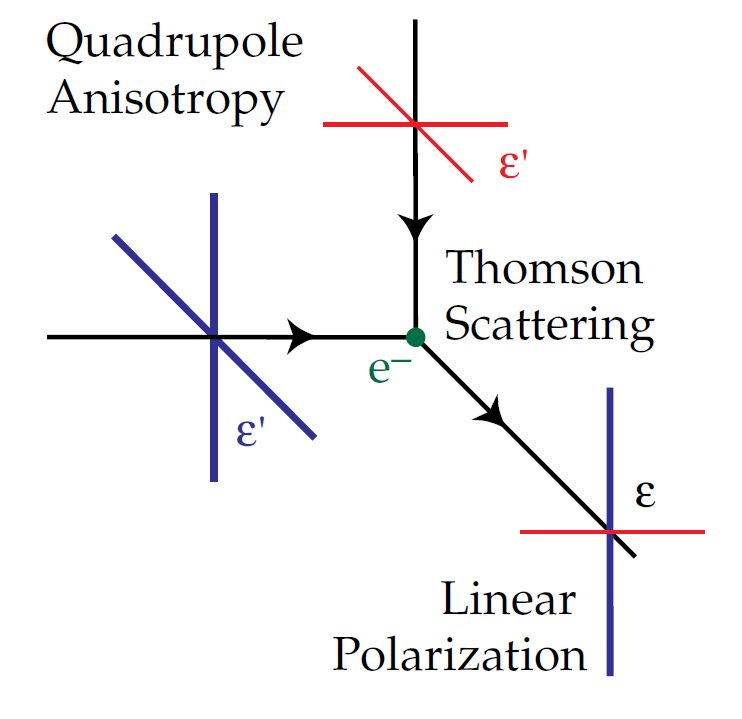
\includegraphics[scale=0.5]{thomson.png}
\caption{Thomson scattering of CMB photons in the presence of a quadrupole anisotropy. The red lines are the polarisations of a cold photon and the blue lines are the polarisations of a hot photon both incident on the same electron. The result is a net linear polarisation.}
\label{fig:thomson}
\end{figure}
\pagebreak
A quadrupole anisotropy can be caused by any of scalar, vector or tensor perturbations. Scalar perturbations are density fluctuations. Vector perturbations result from vortices in the photon-electron fluid or from more exotic phenomena, such as cosmic strings and other topologcal defects. Finally a tensor perturbation would be the result of gravity waves produced during cosmic inflation.  

In order to describe the effects of perturbations on CMB polarisation we introduce two polarisation modes. E-modes and B-modes. E-modes are formed from scalar perturbations. The E-modes resemble electric fields in electromagnetism in the sense that they are curl-free. It is also useful to note that E-modes have even parity. B-modes on the other hand are formed from vector and tensor perturbations and are currently undetected. Continuing the electromagnetism analogy a B-mode resembles a magnetic field, in the sense that it is purely a curl field. B-modes have odd parity.

\begin{SCfigure}
\centering
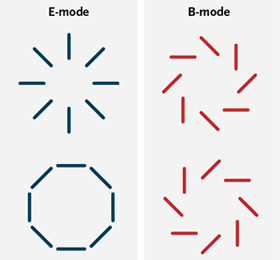
\includegraphics[scale=3]{modes.png}
\caption{Representation of E-mode polarisations and B-mode polarisations. Note how E-modes are symmetric and resemble a divergent field. In contrast the B-modes appear anti-symmetric and resemble a curled field.}
\label{fig:modes}
\end{SCfigure}

The causes of B-mode CMB polarisation are new frontiers in physics. There is a strong case to study CMB polarisation, in the hopes that we may shed some light on the exotic nature of the early Universe.

\subsection{CMB Power Spectrum}

Studies of the CMB often rely on the CMB power spectrum to draw their conclusions. The power spectrum is defined as the amplitude of the Fourier decomposition of a signal given by f(x), like so:

\begin{equation}
P(k) = \vert a_k \vert ^2
\end{equation}
where $a_k$ are the fourier coefficients given by:
\begin{equation}
a_k = \int f(x) e^{-ikx} dx
\end{equation}
However, since the CMB is on the sky, we are required to work in spherical co-ordinates, hence we need to use the angular power spectrum. In spherical co-ordinates all functions can be broken down into spherical harmonics, so some function $T(\hat{n})$ at a point $\hat{n}$, can be written as:
\begin{equation}
T(\hat{n}) = \sum_{\ell = 0}^{\ell_{max}} \sum_{m = -\ell}^{\ell} a_{\ell m} Y_{\ell m}(\hat{n})
\end{equation}
where $a_{lm}$ is once again a fourier coefficient given by:
\begin{equation}
a_{\ell m} = \int_{4 \pi} T(\hat{n}) Y_{\ell m}^{*}(\hat{n})
\end{equation}
The angular power spectrum is then defined as:
\begin{equation}
C_{\ell} = \frac{1}{2\ell + 1} \sum_{m = -\ell}^{\ell} \vert a_{\ell m} \vert ^2
\end{equation}
The $C_{\ell}$s are functions of the angular scales, $\ell$. The angular power sprectrum of the CMB is very sensitive to the conditions of the early Universe and hence a powerful probe of Big Bang Cosmology.

\subsection{CMB-S3}
	- stage 3 of CMB experiments operating from 2016 to 2020.
	- n detectors, m detector years
	- primary science goal is to detect PGW from cosmic inflation through B-modes.
	- could also make a detection of PMFs.
\subsubsection{SPT-3G}
	- South Pole Telescope
	- n detectors
	- starting/finishing dates
	- area
	- etc.
\subsubsection{Advanced ACTPol}
\subsubsection{The Simons Array}
\subsection{CMB-S4}
	- stage 4 CMB experiments still in planning stages - nothing concrete yet.
	- n detectors, m detector years
	- running through the 2020s